\documentclass[12pt,a4paper]{report}
\usepackage{fontspec}
\setmainfont{Times New Roman}

\usepackage[margin=2.2cm,top=2.5cm,bottom=2.5cm]{geometry}
\usepackage{amsmath,amssymb,amsfonts,amsthm}
\usepackage{graphicx}
\usepackage{booktabs}
\usepackage{longtable}
\usepackage{array}
\usepackage{tabularx}
\usepackage{xcolor}
\usepackage{fancyhdr}
\usepackage{hyperref}

\hypersetup{
    colorlinks=true,
    linkcolor=blue!70!black,
    citecolor=green!50!black,
    urlcolor=teal
}

\linespread{1.25}

\pagestyle{fancy}
\fancyhf{}
\fancyhead[L]{\small\itshape Suy luận thống kê (MI3031) -- Nhóm 18}
\fancyhead[R]{\small\itshape Báo cáo cuối kỳ}
\fancyfoot[C]{\thepage}

\begin{document}

% ==================== TRANG BÌA ====================
\begin{titlepage}
\begin{center}
    \vspace*{1.5cm}
    {\Large\bfseries BÁO CÁO BÀI TẬP LỚN}\\[10pt]
    {\Large\bfseries HỌC PHẦN: SUY LUẬN THỐNG KÊ (MI3031)}\\[30pt]

    {\huge\bfseries SUY LUẬN THỐNG KÊ TRÊN DỮ LIỆU GYM}\\[40pt]

    \begin{minipage}{0.85\textwidth}
        \begin{tabular}{ll}
            \textbf{Nhóm thực hiện:} & \textbf{Nhóm 18} \\[6pt]
            \textbf{Thành viên 1:} & \textbf{Nguyễn Thị Thảo} -- MSSV: \textbf{202419101} \\
            \textbf{Thành viên 2:} & \textbf{Nguyễn Văn Nam Khánh} -- MSSV: \textbf{202419069} \\[6pt]
            \textbf{Học kỳ:} & 2026.1 \\[6pt]
            \textbf{GitHub Repository:} & \url{https://github.com/thhaaaoooo2006/SLTK_Nhom-18_Gym-Members-Exercise}
        \end{tabular}
    \end{minipage}

    \vfill
    {\large Hà Nội, Tháng 11 Năm 2026}
\end{center}
\end{titlepage}

% ==================== MỤC LỤC ====================
\pagenumbering{roman}
\tableofcontents
\newpage
\pagenumbering{arabic}

% ==================== LỜI MỞ ĐẦU ====================
\chapter*{Lời mở đầu}
\addcontentsline{toc}{chapter}{Lời mở đầu}
Trong bối cảnh khoa học thể thao hiện đại, việc theo dõi định lượng các chỉ số sinh học và hiệu suất vận động đóng vai trò then chốt trong việc tối ưu hóa giáo án tập luyện, kiểm soát cân nặng và phòng tránh chấn thương. Học phần \textbf{Suy luận Thống kê (MI3031)} cung cấp nền tảng toán học chặt chẽ để từ một tập dữ liệu mẫu quan sát có thể suy diễn và khái quát hóa quy luật của toàn bộ tổng thể.

Báo cáo này nghiên cứu bộ dữ liệu \textbf{Gym Members Exercise Tracking} gồm $n = 973$ thành viên phòng gym với 15 chỉ số thể chất và hành vi. Toàn bộ mã nguồn phân tích được xây dựng bằng ngôn ngữ Python từ các công thức toán học nguyên bản, chỉ sử dụng thư viện \texttt{scipy.stats} để tra cứu các phân vị lý thuyết ($t, F, \chi^2, z$), qua đó làm sáng tỏ các định lý toán học cốt lõi như Định lý Gauss-Markov (BLUE), tính tương đương giữa kiểm định $t$ và $F$ ($t_0^2 = f_0$), kiểm định Fisher $Z$, và nguyên lý ngoại suy trong hồi quy.

% ==================== CHƯƠNG 1 ====================
\chapter{Mẫu ngẫu nhiên và thống kê mô tả}
\section{Cơ sở lý thuyết mẫu ngẫu nhiên}
\subsection{Định nghĩa mẫu ngẫu nhiên và hàm thống kê}
Cho $X$ là một đại lượng ngẫu nhiên đặc trưng cho tổng thể với hàm phân phối xác suất tích lũy $F(x)$ chưa biết.
\begin{itemize}
    \item \textbf{Mẫu ngẫu nhiên}: Bộ $n$ đại lượng ngẫu nhiên $(X_1, X_2, \dots, X_n)$ được gọi là mẫu ngẫu nhiên kích thước $n$ nếu chúng độc lập và có cùng phân phối xác suất với $X$ (iid -- independent and identically distributed):
    \[ P(X_1 \le x_1, X_2 \le x_2, \dots, X_n \le x_n) = \prod_{i=1}^n F(x_i) \]
    \item \textbf{Hàm thống kê}: Mọi hàm thực $T = g(X_1, \dots, X_n)$ hoàn toàn xác định từ các biến ngẫu nhiên mẫu và không chứa tham số tổng thể chưa biết được gọi là hàm thống kê.
\end{itemize}

\subsection{Các đặc trưng mẫu cơ bản}
\begin{enumerate}
    \item \textbf{Trung bình mẫu}:
    \[ \bar{X} = \frac{1}{n}\sum_{i=1}^n X_i \]
    Kỳ vọng $E(\bar{X}) = \mu$, phương sai $Var(\bar{X}) = \frac{\sigma^2}{n}$. $\bar{X}$ là ước lượng không chệch, vững và hiệu quả cho kỳ vọng $\mu$.
    
    \item \textbf{Phương sai mẫu hiệu chỉnh}:
    \[ S^2 = \frac{1}{n-1}\sum_{i=1}^n (X_i - \bar{X})^2 \]
    Việc chia cho bậc tự do $n - 1$ thay vì $n$ là điều kiện toán học bắt buộc để ước lượng không bị chệch: $E(S^2) = \sigma^2$. Nếu chia cho $n$, kỳ vọng chỉ đạt $\frac{n-1}{n}\sigma^2$.
    
    \item \textbf{Độ lệch chuẩn mẫu hiệu chỉnh}: $S = \sqrt{S^2}$.
    
    \item \textbf{Tần suất mẫu}:
    \[ \hat{p} = \frac{k}{n} = \frac{1}{n}\sum_{i=1}^n I_A(X_i) \]
    với $k$ là số phần tử thỏa biến cố $A$, là ước lượng không chệch cho xác suất $p$ của tổng thể.
\end{enumerate}

\section{Bối cảnh dữ liệu và tiền xử lý}
Bộ dữ liệu gồm $973$ dòng quan sát và $15$ cột biến thuộc 3 nhóm:
\begin{itemize}
    \item \textbf{Định lượng liên tục}: Weight (kg), Height (m), Session\_Duration (giờ), Calories\_Burned (kcal), Fat\_Percentage (\%), Water\_Intake (lít), BMI.
    \item \textbf{Định lượng rời rạc}: Age, Max\_BPM, Avg\_BPM, Resting\_BPM, Workout\_Frequency.
    \item \textbf{Định tính / Phân loại}: Gender (Male: 511, Female: 462), Workout\_Type (Cardio, HIIT, Strength, Yoga), Experience\_Level (1, 2, 3).
\end{itemize}

\textbf{Chất lượng dữ liệu}: Kiểm tra toàn diện cho thấy $0$ giá trị khuyết thiếu (Missing = 0) và $0$ dòng dữ liệu trùng lặp (Duplicate = 0). Áp dụng phương pháp Tukey IQR Fences ($[Q_1 - 1.5 IQR, Q_3 + 1.5 IQR]$), các giá trị ngoại lai ghi nhận ở lượng calo hoặc BMI đều phản ánh vận động viên thể hình thực tế nên được giữ nguyên nhằm bảo đảm tính khách quan.

\section{Bảng thống kê mô tả thực nghiệm}
\begin{table}[htbp]
\centering\small
\caption{Thống kê mô tả các biến định lượng trọng tâm ($n = 973$)}
\begin{tabular}{lrrrrrr}
\toprule
\textbf{Biến} & \textbf{Trung bình ($\bar{x}$)} & \textbf{Phương sai ($S^2$)} & \textbf{Độ lệch chuẩn ($S$)} & \textbf{Trung vị} & \textbf{Min} & \textbf{Max} \\
\midrule
Calories\_Burned & 905.4224 & 74333.3965 & 272.6415 & 893.00 & 285.00 & 1650.00 \\
Session\_Duration & 1.2564 & 0.1177 & 0.3430 & 1.25 & 0.50 & 2.00 \\
Avg\_BPM & 143.4358 & 232.0624 & 15.2336 & 143.00 & 120.00 & 170.00 \\
Weight (kg) & 73.0874 & 225.1051 & 15.0035 & 72.80 & 40.00 & 115.00 \\
Fat\_Percentage & 24.9353 & 38.6475 & 6.2167 & 24.90 & 10.00 & 35.00 \\
\bottomrule
\end{tabular}
\end{table}

% ==================== CHƯƠNG 2 ====================
\chapter{Ước lượng tham số}
\section{Cơ sở lý thuyết ước lượng}
\subsection{Ước lượng điểm: phương pháp mô-men và hợp lý cực đại}
\begin{itemize}
    \item \textbf{Kỳ vọng $\mu$}: Cả MoM và MLE của $\mu$ đều dẫn đến trung bình mẫu $\hat{\mu} = \bar{X}$, là ước lượng không chệch và có phương sai nhỏ nhất trong lớp ước lượng tuyến tính (MVUE).
    \item \textbf{Phương sai $\sigma^2$}: MLE cho phương sai là $\hat{\sigma}^2_{MLE} = \frac{1}{n}\sum (X_i - \bar{X})^2$, bị chệch dưới. Nhân với hệ số $\frac{n}{n-1}$ ta được ước lượng không chệch hiệu chỉnh $S^2$.
    \item \textbf{Tỷ lệ $p$}: $\hat{p} = \frac{k}{n}$, đồng thời là ước lượng MoM và MLE của phân phối Bernoulli.
\end{itemize}

\subsection{Khoảng tin cậy 95\%}
Khoảng tin cậy hai phía mức $(1-\alpha)$ cho tham số $\theta$ thỏa mãn $P(\theta_L \le \theta \le \theta_U) = 1 - \alpha$.
\begin{itemize}
    \item KTC cho $\mu$ khi $\sigma$ chưa biết: $\bar{X} \pm t_{\alpha/2, n-1} \frac{S}{\sqrt{n}}$.
    \item KTC cho $\sigma^2$: $\left[\frac{(n-1)S^2}{\chi^2_{\alpha/2, n-1}}, \frac{(n-1)S^2}{\chi^2_{1-\alpha/2, n-1}}\right]$.
    \item KTC cho $p$ (Wald): $\hat{p} \pm z_{\alpha/2} \sqrt{\frac{\hat{p}(1-\hat{p})}{n}}$.
    \item So sánh 2 tổng thể: Sử dụng kiểm định tỷ số phương sai $F = S_1^2 / S_2^2$ trước khi áp dụng công thức $t$-Welch (nếu phương sai khác nhau) hoặc $t$-gộp (nếu phương sai đồng nhất).
\end{itemize}

\section{Kết quả thực nghiệm trên dữ liệu gym}
\begin{table}[htbp]
\centering\small
\caption{Bảng khoảng tin cậy 95\% cho các tham số trọng tâm}
\begin{tabular}{lcccc}
\toprule
\textbf{Tham số} & \textbf{Phương pháp} & \textbf{Ước lượng điểm} & \textbf{KTC 95\% (Hai phía)} \\
\midrule
$\mu$ (Calories\_Burned) & $t$-Student ($df=972$) & 905.4224 & [888.2700, 922.5748] \\
$\sigma^2$ (Session\_Duration) & Chi-bình phương ($df=972$) & 0.1177 & [0.1079, 0.1289] \\
$\sigma$ (Session\_Duration) & $\sqrt{\text{Chi-bình phương}}$ & 0.3430 & [0.3284, 0.3590] \\
$p$ (Gender = Male) & Xấp xỉ chuẩn (Wald) & 0.5252 & [0.4938, 0.5566] \\
$\sigma_1^2 / \sigma_2^2$ (Calories) & $F$-Fisher ($df=510, 461$) & 1.3182 & [1.1024, 1.5749] \\
$\mu_1 - \mu_2$ (Male -- Female) & $t$-Welch ($df=969.67$) & 82.2071 & [48.4674, 115.9467] \\
$p_1 - p_2$ (Tỷ lệ Calo $\ge 1000$) & Xấp xỉ chuẩn (Wald) & 0.1324 & [0.0735, 0.1912] \\
\bottomrule
\end{tabular}
\end{table}

\textbf{Diễn giải tần suất}: Mức tin cậy 95\% có ý nghĩa rằng nếu tiến hành lặp lại quy trình lấy mẫu ngẫu nhiên độc lập 973 thành viên một số lượng rất lớn lần, thì trung bình khoảng 95\% các khoảng tin cậy được tính toán sẽ bao bọc giá trị tham số thực của tổng thể.

% ==================== CHƯƠNG 3 ====================
\chapter{Kiểm định giả thuyết thống kê}
\section{Quy trình kiểm định và ba cách tiếp cận}
Mọi bài toán kiểm định giả thuyết đều được tiến hành qua 5 bước nghiêm ngặt:
(1) Thiết lập cặp giả thuyết $H_0$ và $H_1$; (2) Chọn mức ý nghĩa $\alpha = 0.05$; (3) Xây dựng thống kê kiểm định $T$ và xác định phân phối dưới $H_0$; (4) Tính giá trị thống kê $t_{obs}$ và $P$-value; (5) Kết luận bác bỏ hoặc không bác bỏ $H_0$.

\textbf{Tính nhất quán của 3 cách tiếp cận}: Miền bác bỏ cổ điển ($t_{obs} \in W_\alpha$), $P$-value ($P \le \alpha$) và Đối chiếu KTC ($95\%$ KTC không chứa $\theta_0$) đều cho kết luận hoàn toàn tương đương trên mọi kiểm định thực nghiệm.

\section{Kết quả kiểm định tham số 1 và 2 tổng thể}
\begin{table}[htbp]
\centering\footnotesize
\caption{Tổng hợp kết quả kiểm định tham số mức $\alpha = 0.05$}
\begin{tabularx}{\textwidth}{lccccc}
\toprule
\textbf{Kiểm định} & \textbf{Giả thuyết $H_0$} & \textbf{Thống kê} & \textbf{$P$-value} & \textbf{Kết luận} & \textbf{Nhất quán} \\
\midrule
1. Kỳ vọng Calories & $\mu = 900$ & $T = 0.6204$ & 0.5352 & Không bác bỏ $H_0$ & Có \\
2. Phương sai Thời lượng & $\sigma^2 = 0.10$ & $\chi^2 = 1143.77$ & 0.0002 & Bác bỏ $H_0$ & Có \\
3. Tỷ lệ Nam giới & $p = 0.50$ & $Z = 1.5709$ & 0.1162 & Không bác bỏ $H_0$ & Có \\
4. So sánh 2 phương sai & $\sigma_1^2 = \sigma_2^2$ & $F = 1.3182$ & 0.0025 & Bác bỏ $H_0$ ($\sigma_1^2 \ne \sigma_2^2$) & Có \\
5. So sánh 2 kỳ vọng & $\mu_1 = \mu_2$ & $T_W = 4.7814$ & $2.01 \times 10^{-6}$ & Bác bỏ $H_0$ ($\mu_1 > \mu_2$) & Có \\
6. So sánh 2 tỷ lệ Calo & $p_1 = p_2$ & $Z = 4.3455$ & $1.39 \times 10^{-5}$ & Bác bỏ $H_0$ ($p_1 > p_2$) & Có \\
\bottomrule
\end{tabularx}
\end{table}

\section{ANOVA một nhân tố và kiểm định phi tham số}
\subsection{Phân tích phương sai một nhân tố}
Kiểm định giả thuyết về sự bằng nhau của kỳ vọng calo tiêu thụ giữa 4 loại hình bài tập: $H_0: \mu_{\text{Cardio}} = \mu_{\text{HIIT}} = \mu_{\text{Strength}} = \mu_{\text{Yoga}}$.
\begin{table}[htbp]
\centering\small
\caption{Bảng ANOVA so sánh Calories\_Burned theo Workout\_Type}
\begin{tabular}{lrrrrr}
\toprule
\textbf{Nguồn biến thiên} & \textbf{SS} & \textbf{df} & \textbf{MS} & \textbf{Thống kê $F$} & \textbf{$P$-value} \\
\midrule
Giữa các nhóm (SSF) & 1,481,280.95 & 3 & 493,760.32 & 6.7644 & $0.00016$ \\
Nội bộ nhóm (SSE) & 70,770,775.14 & 969 & 73,034.86 & -- & -- \\
Tổng cộng (SST) & 72,252,056.09 & 972 & -- & -- & -- \\
\bottomrule
\end{tabular}
\end{table}
Do $F = 6.7644 > F_{0.05, 3, 969} = 2.6141$ ($P = 0.00016 < 0.05$), ta \textbf{bác bỏ $H_0$}. Loại hình bài tập có tác động thực sự đến lượng calo tiêu hao (HIIT và Cardio đạt trung bình calo cao nhất).

\subsection{Kiểm định phi tham số chi-bình phương}
\begin{enumerate}
    \item \textbf{Kiểm định chi-bình phương phù hợp phân phối chuẩn}:
    Với $k = 10$ khoảng phân lớp ($df = k - 1 - 2 = 7$), Session\_Duration đạt $\chi^2 = 2.4578$ ($P = 0.9303 > 0.05$), không bác bỏ giả thuyết phân phối chuẩn. Calories\_Burned đạt $\chi^2 = 5.2140$ ($P = 0.6338 > 0.05$), hoàn toàn phù hợp với phân phối chuẩn.
    \item \textbf{Kiểm định tính độc lập giữa giới tính và cấp độ kinh nghiệm}:
    Bảng tiếp biến $2 \times 3$ ($df = (2-1)(3-1) = 2$) cho giá trị thống kê $\chi^2 = 0.0128$, giá trị tới hạn $\chi^2_{0.05, 2} = 5.9915$, $P = 0.9936$. Kết luận \textbf{không bác bỏ $H_0$}: Giới tính và Trình độ kinh nghiệm tập luyện hoàn toàn độc lập với nhau.
\end{enumerate}

% ==================== CHƯƠNG 4 ====================
\chapter{Hồi quy tuyến tính và tương quan}
\section{Mô hình hồi quy tuyến tính đơn OLS}
Mô hình toán học: $Y_i = \beta_0 + \beta_1 X_i + \varepsilon_i$, với $Y$: Calories\_Burned, $X$: Session\_Duration.
Các giả thiết Gauss-Markov: $E(\varepsilon_i) = 0$, $Var(\varepsilon_i) = \sigma^2$, $Cov(\varepsilon_i, \varepsilon_j) = 0$ ($i \ne j$), $\varepsilon_i \sim \mathcal{N}(0, \sigma^2)$.

\begin{table}[htbp]
\centering\small
\caption{Hệ số hồi quy và kiểm định giả thuyết ($n = 973$)}
\begin{tabular}{lrrrrr}
\toprule
\textbf{Hệ số} & \textbf{Ước lượng} & \textbf{Sai số chuẩn $SE$} & \textbf{Thống kê $t$} & \textbf{$P$-value} & \textbf{KTC 95\%} \\
\midrule
$\beta_0$ (Hệ số chặn) & $-1.4465$ & 13.9074 & $-0.104$ & 0.9172 & [$-28.7385$, 25.8455] \\
$\beta_1$ (Thời lượng) & 721.7860 & 10.6786 & 67.592 & $< 10^{-15}$ & [700.8303, 742.7418] \\
\bottomrule
\end{tabular}
\end{table}

Phương trình hồi quy thực nghiệm:
\[ \hat{y} = -1.45 + 721.79 \cdot x \]
Hệ số góc $\hat{\beta}_1 = 721.79$ có ý nghĩa: khi thời lượng tập tăng thêm 1 giờ, lượng calo đốt cháy trung bình tăng thêm xấp xỉ 721.8 kcal.

\section{ANOVA hồi quy và chứng minh tương đương $t_0^2 = f_0$}
\begin{table}[htbp]
\centering\small
\caption{Bảng ANOVA mô hình hồi quy tuyến tính đơn}
\begin{tabular}{lrrrrr}
\toprule
\textbf{Nguồn biến thiên} & \textbf{SS} & \textbf{df} & \textbf{MS} & \textbf{Thống kê $F$} & \textbf{$P$-value} \\
\midrule
Hồi quy (SSR) & 59,587,640.71 & 1 & 59,587,640.71 & 4568.6744 & $< 10^{-15}$ \\
Sai số phần dư (SSE) & 12,664,415.38 & 971 & 13,042.65 & -- & -- \\
Tổng cộng (SST) & 72,252,056.09 & 972 & -- & -- & -- \\
\bottomrule
\end{tabular}
\end{table}

\textbf{Chứng minh tính tương đương toán học $t_0^2 = f_0$}:
Trong hồi quy đơn, thống kê kiểm định $t$ cho hệ số góc là $t_0 = \frac{\hat{\beta}_1}{s / \sqrt{S_{xx}}}$. Khi bình phương:
\[ t_0^2 = \frac{\hat{\beta}_1^2 S_{xx}}{s^2} = \frac{SSR}{s^2} = \frac{MSR}{MSE} = f_0 \]
Thực nghiệm số liệu: $t_0^2 = (67.591969)^2 = 4568.6744 = f_0$. Do đó kiểm định $t$ và kiểm định $F$ cho hệ số góc là hoàn toàn tương đương.
Hệ số xác định $R^2 = \frac{SSR}{SST} = 0.8247$ ($82.47\%$ biến thiên lượng calo được giải thích tuyến tính bởi thời lượng tập).

\section{Khoảng tin cậy cho kỳ vọng và khoảng dự đoán cho cá thể}
\begin{itemize}
    \item KTC cho kỳ vọng phản hồi $E(Y|x_0)$: $\hat{y}_0 \pm t_{\alpha/2, n-2} \cdot s \sqrt{\frac{1}{n} + \frac{(x_0 - \bar{x})^2}{S_{xx}}}$.
    \item Khoảng dự đoán cho quan sát mới $Y_0$: $\hat{y}_0 \pm t_{\alpha/2, n-2} \cdot s \sqrt{1 + \frac{1}{n} + \frac{(x_0 - \bar{x})^2}{S_{xx}}}$.
\end{itemize}
Khoảng dự đoán luôn rộng hơn KTC do có thêm số hạng ``$+1$'' biểu thị phương sai ngẫu nhiên của chính cá thể mới ($Var(y_0 - \hat{y}_0) = Var(\hat{y}_0) + \sigma^2$).

\begin{figure}[htbp]
\centering
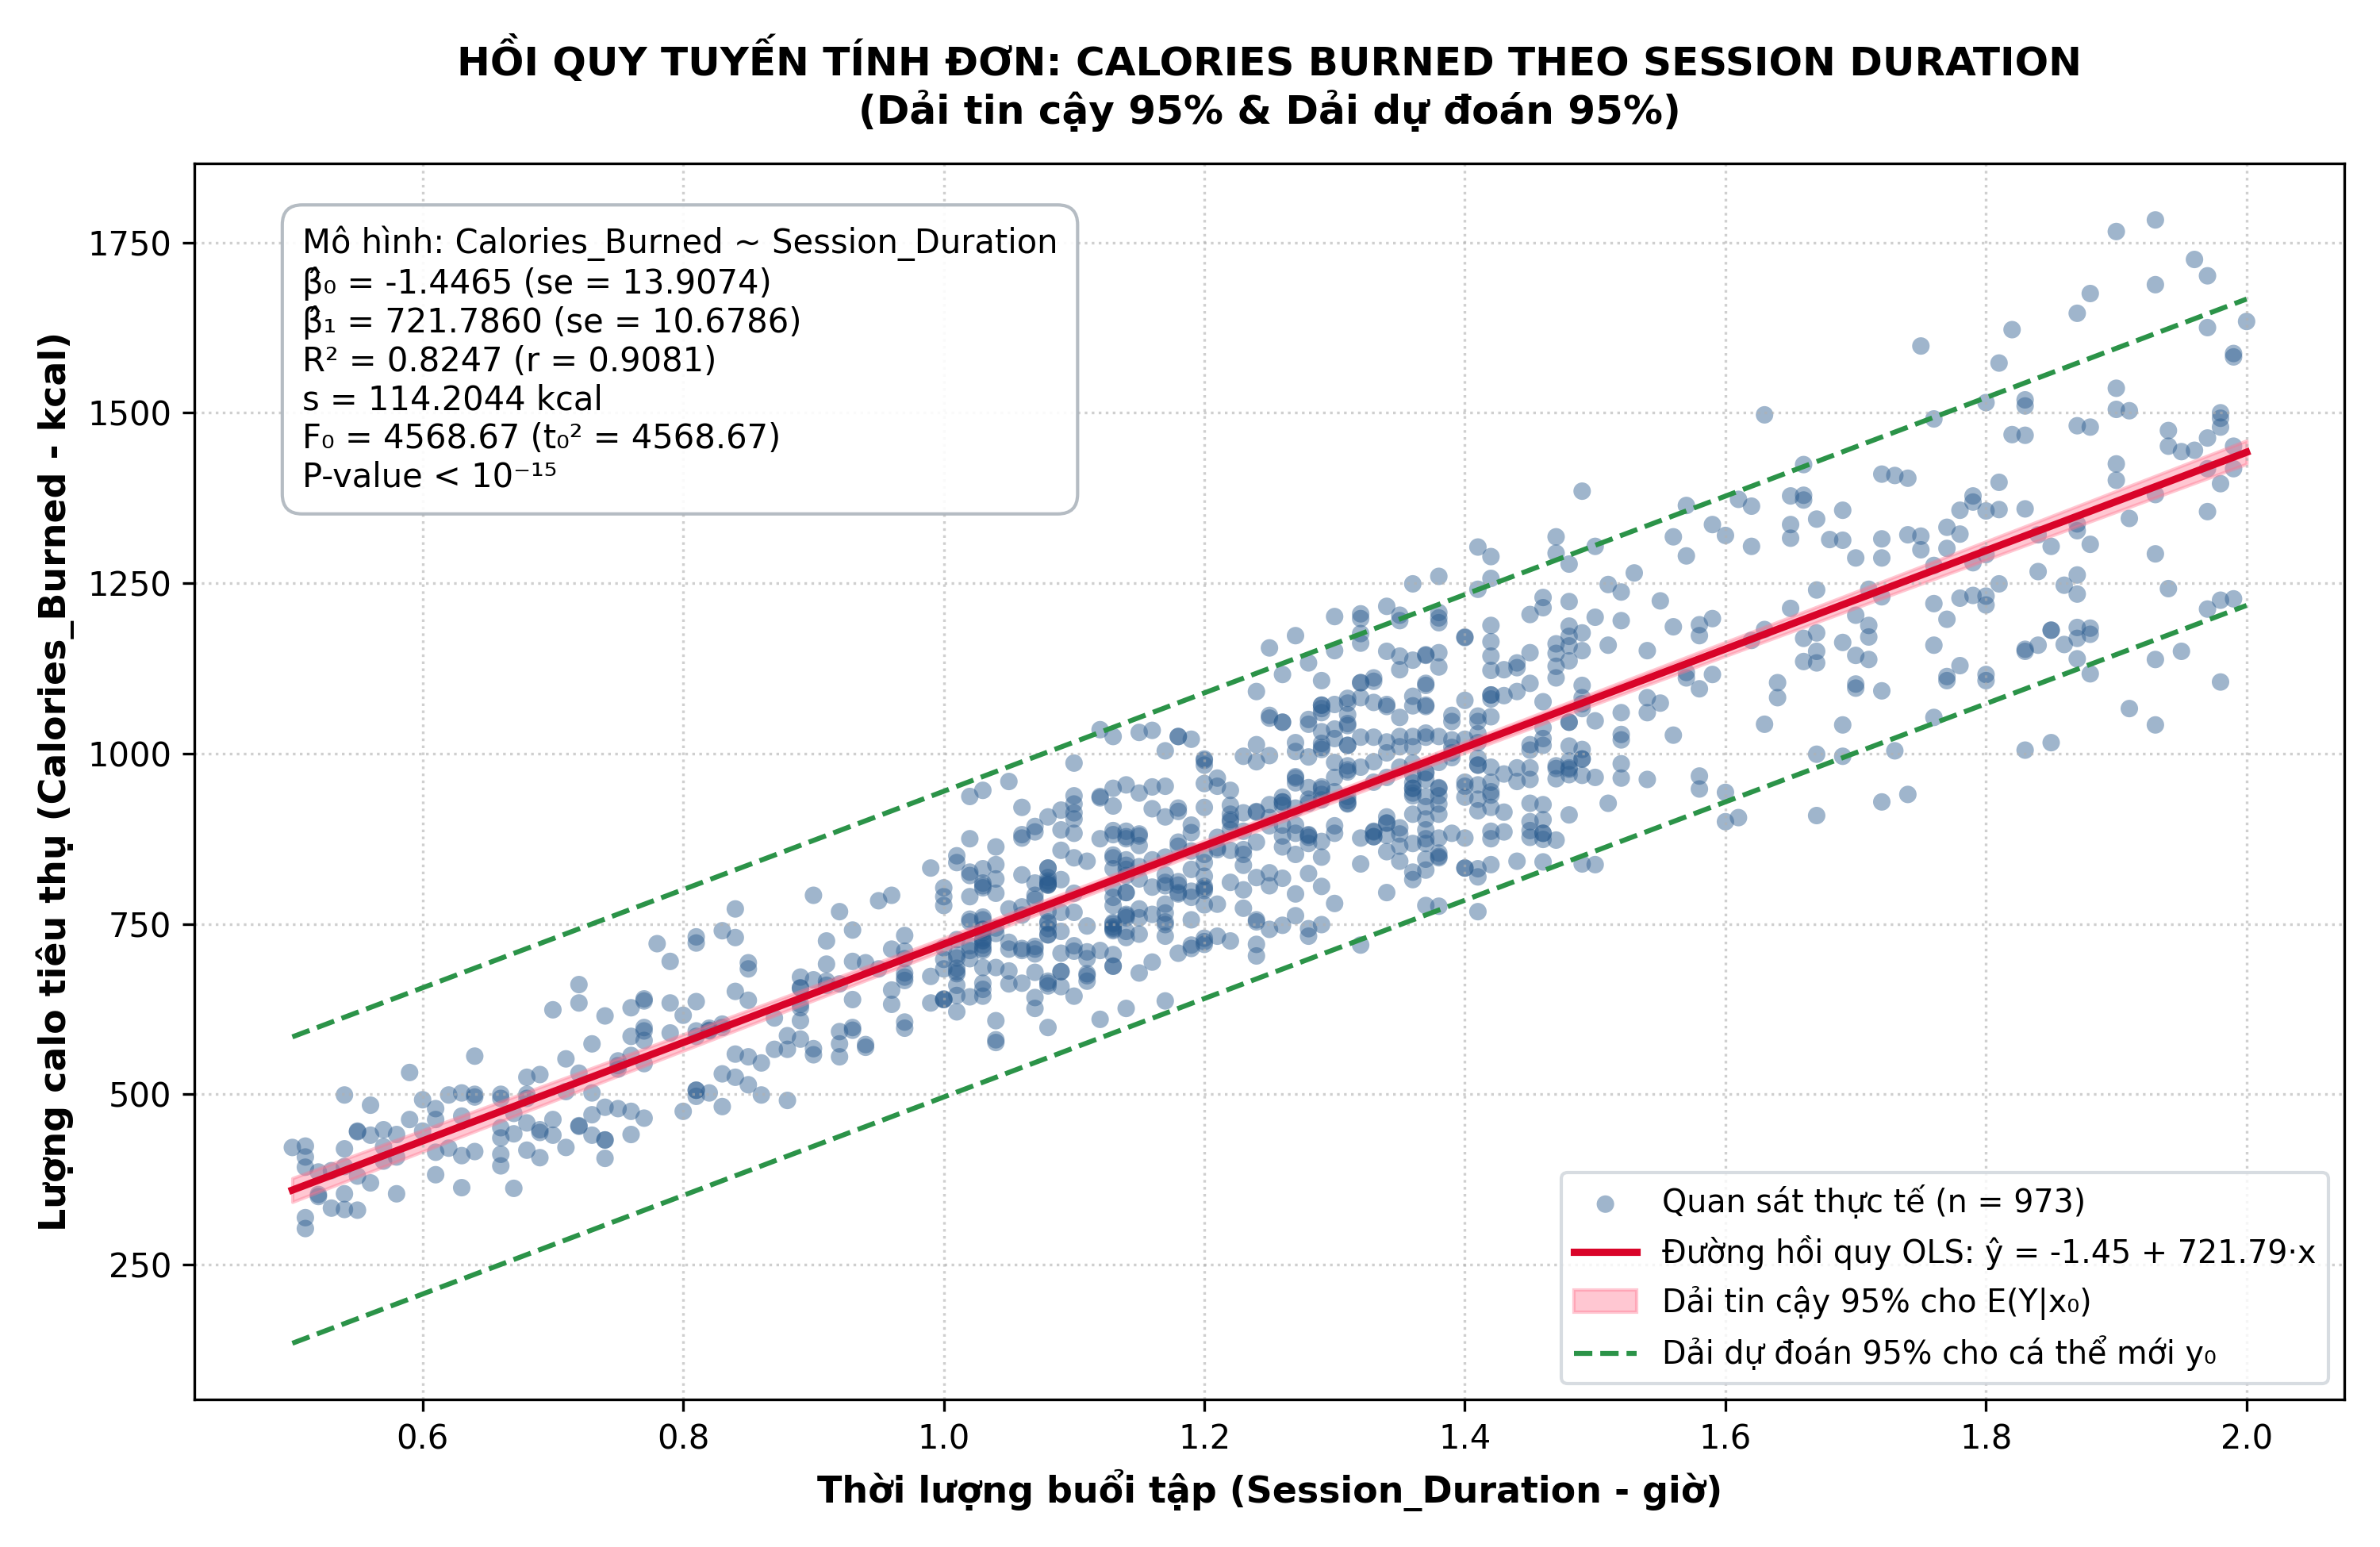
\includegraphics[width=0.92\textwidth]{../outputs/figures/05_slr_bands.png}
\caption{Đồ thị hồi quy tuyến tính đơn với dải tin cậy 95\% và dải dự đoán 95\%}
\end{figure}

\section{Ý nghĩa thực tế của hệ số chặn $\hat{\beta}_0$}
\begin{itemize}
    \item \textbf{Về mặt thực tế}: Trong mẫu quan sát, thời lượng tập $x \in [0.5, 2.0]$ giờ. Không có ai tập 0 giờ. Việc diễn giải máy móc ``tập 0 giờ đốt $-1.45$ kcal'' là sai lầm ngoại suy (Extrapolation).
    \item \textbf{Về mặt toán học}: $\hat{\beta}_0$ đóng vai trò \textbf{mỏ neo toán học} bắt buộc: (1) Đảm bảo tổng phần dư $\sum e_i = 0$; (2) Buộc đường hồi quy đi qua trọng tâm mẫu $(\bar{x}, \bar{y})$; (3) Đảm bảo phân rã $SST = SSR + SSE$ và $R^2 \in [0, 1]$.
\end{itemize}

\section{Phân tích phần dư và chẩn đoán mô hình}
Đồ thị chẩn đoán 4 bảng được thể hiện trong Hình \ref{fig:res_diag}. Phần dư phân tán đều thành dải băng quanh 0 (Homoscedasticity), Q-Q plot bám sát đường 45° khẳng định giả thiết phân phối chuẩn không bị vi phạm.
\begin{figure}[htbp]
\centering
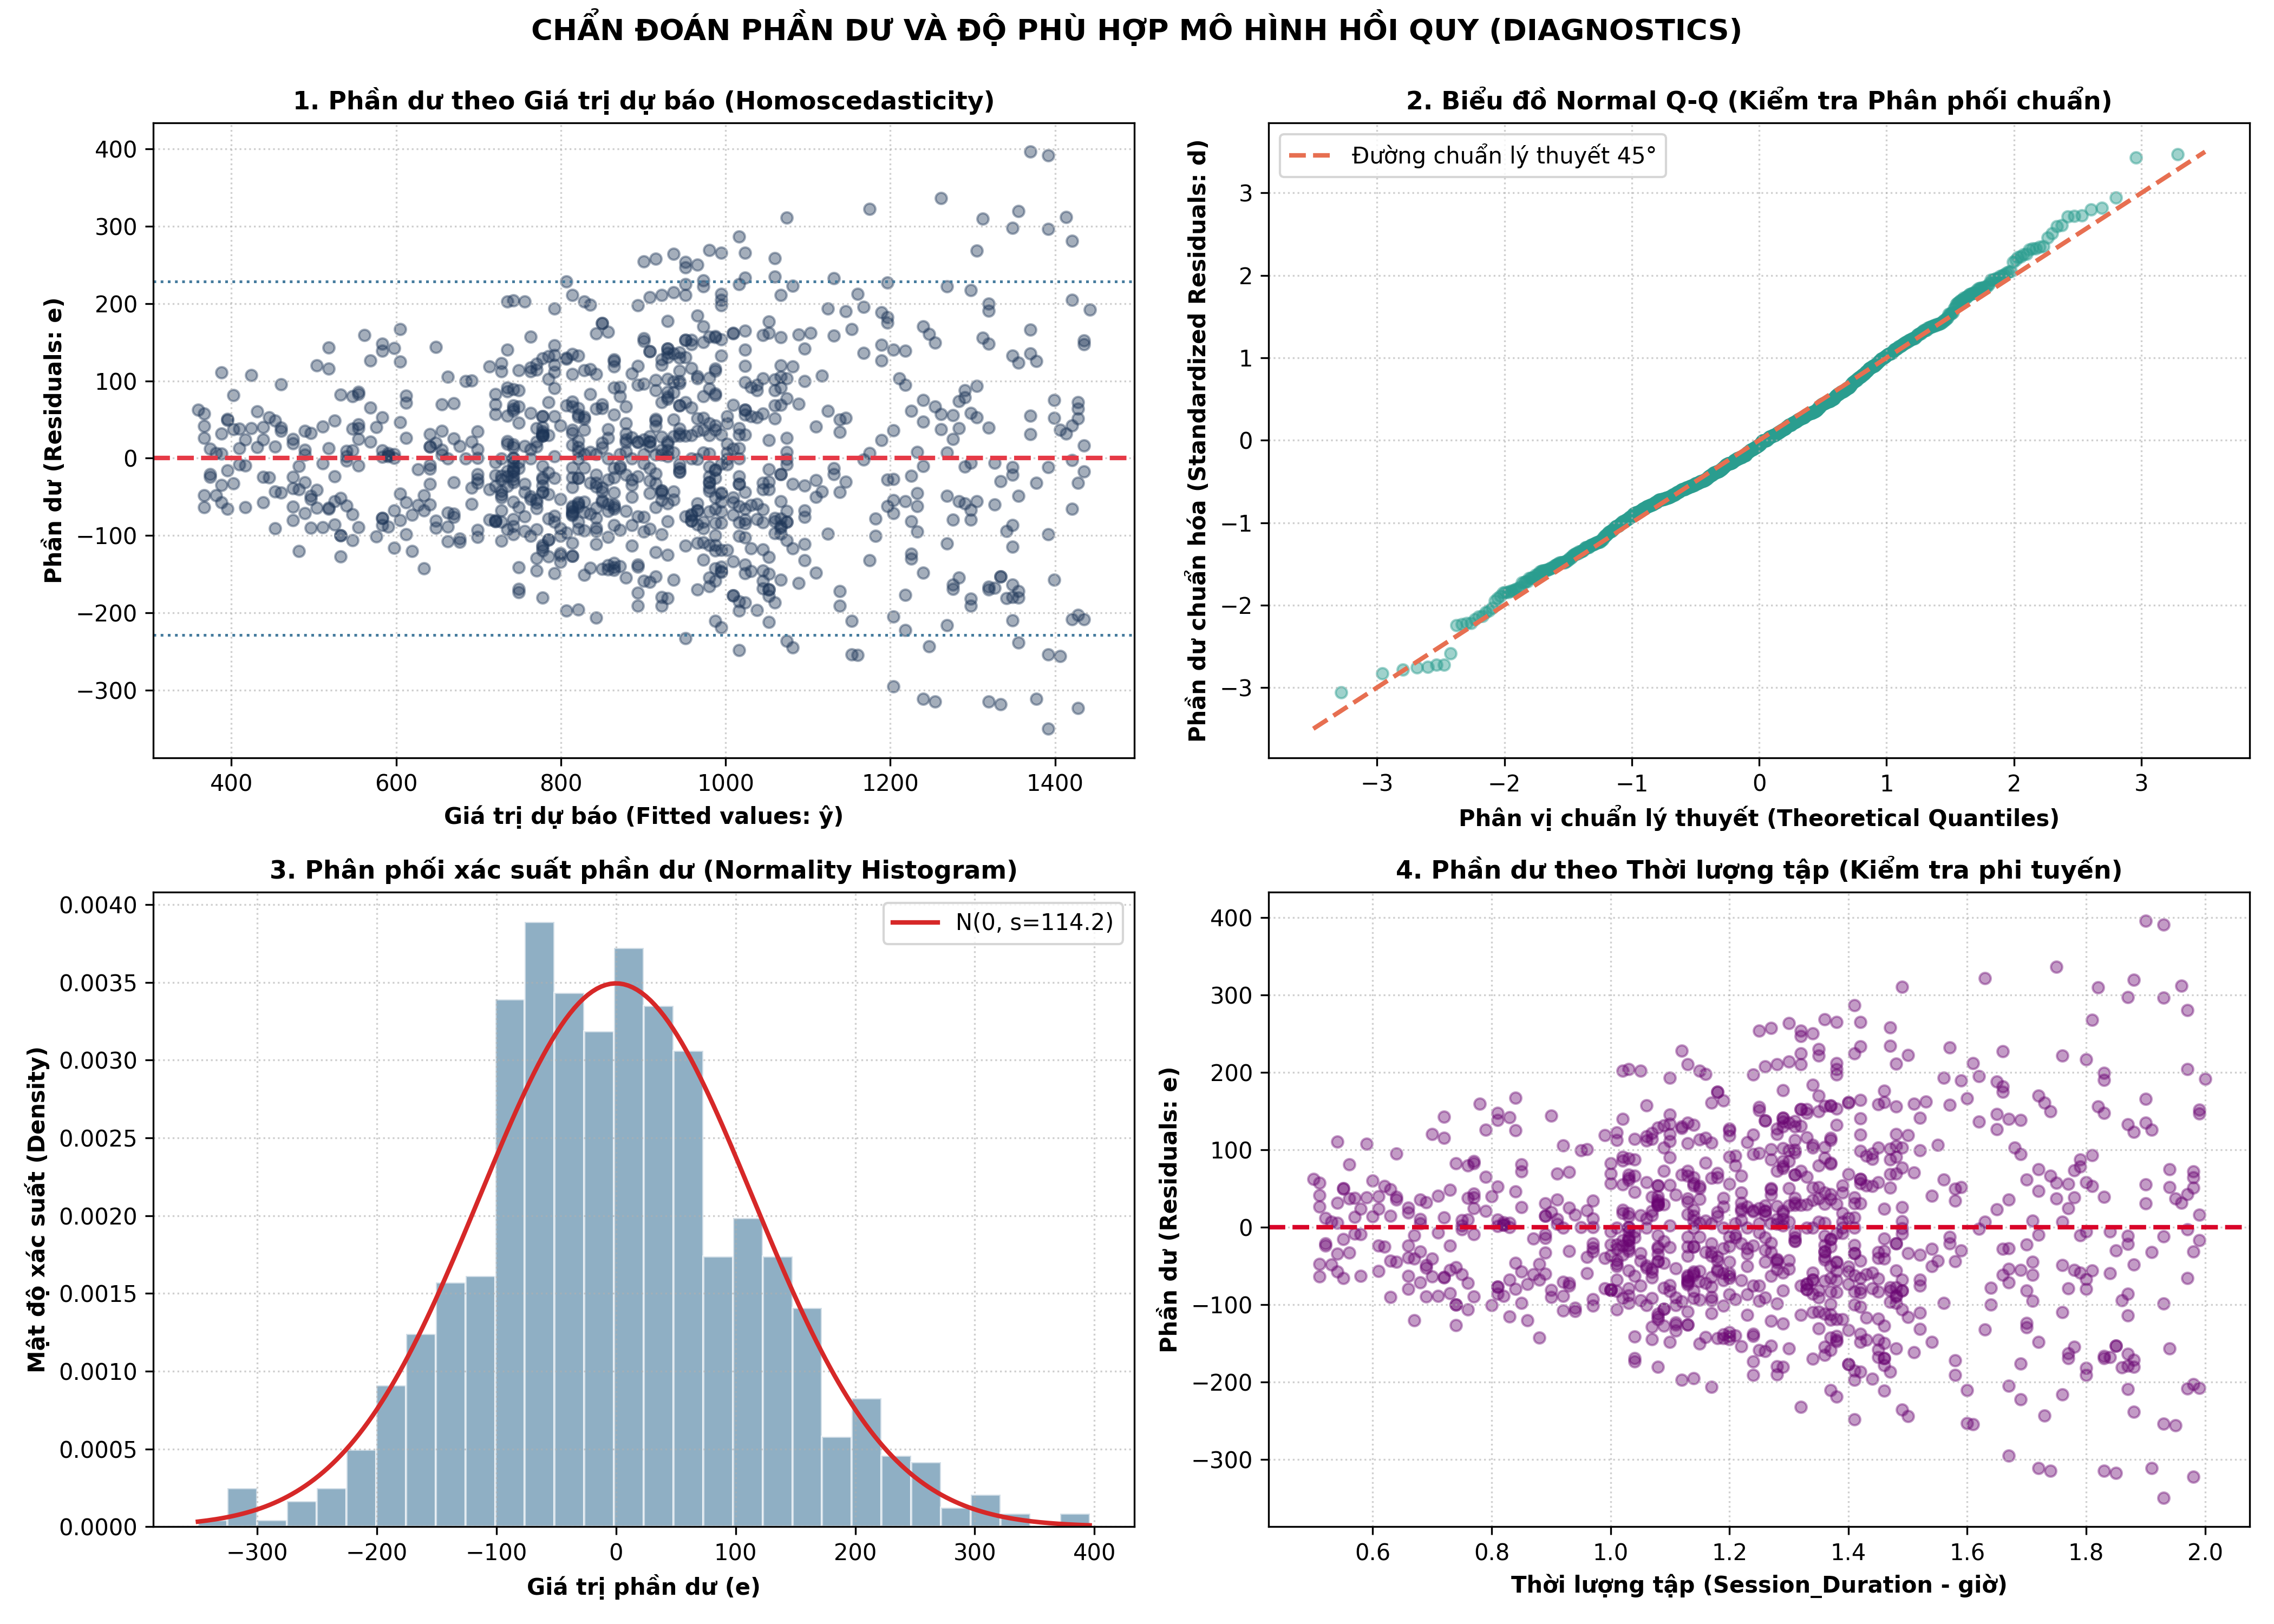
\includegraphics[width=0.92\textwidth]{../outputs/figures/06_residual_diagnostics.png}
\caption{Bộ 4 biểu đồ chẩn đoán phần dư và kiểm tra giả thiết Gauss-Markov}
\label{fig:res_diag}
\end{figure}

\section{Hệ số tương quan Pearson và biến đổi Fisher Z}
Hệ số tương quan mẫu $r = 0.9081$ (đồng biến rất mạnh).
\begin{itemize}
    \item Kiểm định $H_0: \rho = 0$: $t_0 = 67.592$, $P < 10^{-15}$ $\rightarrow$ Bác bỏ $H_0$.
    \item Kiểm định $H_0: \rho = 0.85$ qua biến đổi Fisher $Z = \text{arctanh}(r) = 1.5167$: $Z_0 = 8.1633 > 1.96$ ($P < 10^{-15}$) $\rightarrow$ Bác bỏ $H_0$, $\rho$ thực tế cao hơn $0.85$.
    \item KTC 95\% cho $\rho$: $[0.8965, 0.9185]$.
\end{itemize}

\textbf{Tương quan không đồng nghĩa với Nhân quả}: Mặc dù $r$ rất cao, thời lượng tập không phải nguyên nhân duy nhất quyết định lượng calo. Các biến can thiệp (Confounding variables) như nhịp tim trung bình (\texttt{Avg\_BPM}), khối lượng cơ thể (\texttt{Weight}) và loại bài tập (\texttt{Workout\_Type}) cùng đóng vai trò chi phối, đòi hỏi cần mở rộng sang mô hình Hồi quy bội.

\section{Hồi quy tuyến tính bội và phương pháp ước lượng bình phương nhỏ nhất}
\subsection{Giới thiệu về mô hình hồi quy tuyến tính bội (Mục 4.3.1)}
Mô hình hồi quy tuyến tính đơn chỉ đánh giá tác động của một biến độc lập $x$ lên giá trị trung bình của biến phụ thuộc $Y$, do đó dễ vi phạm Giả thiết 1(2) về sai số ngẫu nhiên khi vẫn còn nhiều yếu tố khác cùng tác động đến $Y$. Điều này dẫn đến sự cần thiết của \textbf{mô hình hồi quy tuyến tính bội} (còn gọi là mô hình hồi quy bội hay hồi quy đa biến).

Trong trường hợp tổng quát với $k$ biến độc lập (biến hồi quy, biến giải thích) $x_1, x_2, \dots, x_k$, mô hình hồi quy tuyến tính bội có dạng:
\[
    Y = \beta_0 + \sum_{j=1}^{k} \beta_j x_j + \varepsilon
\]
trong đó $\beta_0$ là \textbf{hệ số chặn}, $\beta_1, \dots, \beta_k$ là \textbf{các hệ số góc} chưa biết (còn gọi là \textbf{các hệ số hồi quy riêng} hay \textbf{các hệ số hồi quy lý thuyết}), và $\varepsilon$ là \textbf{sai số ngẫu nhiên} đại diện cho các yếu tố ngoài $x_1, \dots, x_k$ có tác động đến $Y$ nhưng chưa đưa vào mô hình. Với giả thiết $E(\varepsilon) = 0$, \textbf{hàm hồi quy tuyến tính lý thuyết} của $Y$ theo $k$ biến là:
\[
    E(Y \mid x_1, \dots, x_k) = \beta_0 + \sum_{j=1}^{k} \beta_j x_j
\]
Về mặt hình học, mô hình với $k = 2$ biến hồi quy mô tả một \textbf{mặt phẳng hồi quy} trong không gian ba chiều của $(Y, x_1, x_2)$ với các \textbf{đường đồng mức} (các đường có hằng số $E(Y)$) là các đường thẳng; còn mô hình tổng quát với $k$ biến mô tả một \textbf{siêu phẳng} trong không gian $k$-chiều của $\{x_j\}$. Hệ số hồi quy riêng $\beta_j$ ($j = 1, \dots, k$) biểu thị sự thay đổi dự kiến (kỳ vọng) trong phản hồi $Y$ trên mỗi đơn vị thay đổi trong $x_j$ khi tất cả các biến hồi quy còn lại $x_i$ ($i \ne j$) được giữ không đổi.

Ngoài ra, các mô hình có \textbf{hiệu ứng tương tác} giữa hai biến $x_1$ và $x_2$ được biểu diễn bằng thuật ngữ tích chéo $x_1 x_2$:
\[
    Y = \beta_0 + \beta_1 x_1 + \beta_2 x_2 + \beta_{12} x_1 x_2 + \varepsilon
\]
vẫn là một mô hình hồi quy tuyến tính bội vì tuyến tính theo các tham số $\beta$ (bằng cách đặt $x_3 = x_1 x_2$ và $\beta_3 = \beta_{12}$). Hiệu ứng tương tác ngụ ý rằng tác động gây ra bởi việc thay đổi $x_1$ phụ thuộc vào mức độ của biến $x_2$, làm cho các đường đồng mức trên mặt phẳng $(x_1, x_2)$ bị uốn cong thay vì là đường thẳng.

\subsection{Phương pháp ước lượng bình phương nhỏ nhất (Mục 4.3.2)}
Giả sử có $k$ biến hồi quy và $n > k$ quan sát $(x_{i1}, x_{i2}, \dots, x_{ik}; y_i)$, $i = 1, 2, \dots, n$, với $x_{ij}$ biểu thị quan sát thứ $i$ (hoặc mức độ) của biến $x_j$. Mỗi quan sát thỏa mãn:
\[
    y_i = \beta_0 + \beta_1 x_{i1} + \beta_2 x_{i2} + \dots + \beta_k x_{ik} + \varepsilon_i = \beta_0 + \sum_{j=1}^{k} \beta_j x_{ij} + \varepsilon_i, \quad i = 1, 2, \dots, n.
\]
\textbf{Hàm bình phương nhỏ nhất} được xác định bởi:
\[
    L = \sum_{i=1}^{n} \varepsilon_i^2 = \sum_{i=1}^{n} \left( y_i - \beta_0 - \sum_{j=1}^{k} \beta_j x_{ij} \right)^2
\]
Để cực tiểu hóa $L$ đối với $\beta_0, \beta_1, \dots, \beta_k$, các ước lượng bình phương nhỏ nhất $\hat{\beta}_0, \hat{\beta}_1, \dots, \hat{\beta}_k$ phải thỏa mãn điều kiện đạo hàm riêng bằng $0$:
\[
    \left.\frac{\partial L}{\partial \beta_0}\right|_{\hat{\beta}_0, \dots, \hat{\beta}_k} = -2\sum_{i=1}^{n}\left( y_i - \hat{\beta}_0 - \sum_{j=1}^{k} \hat{\beta}_j x_{ij} \right) = 0
\]
\[
    \left.\frac{\partial L}{\partial \beta_j}\right|_{\hat{\beta}_0, \dots, \hat{\beta}_k} = -2\sum_{i=1}^{n}\left( y_i - \hat{\beta}_0 - \sum_{l=1}^{k} \hat{\beta}_l x_{il} \right) x_{ij} = 0, \quad j = 1, \dots, k.
\]
Rút gọn các phương trình trên thu được hệ $p = k + 1$ \textbf{phương trình chuẩn bình phương nhỏ nhất}:
\[
\begin{cases}
    n\hat{\beta}_0 + \hat{\beta}_1 \sum_{i=1}^n x_{i1} + \hat{\beta}_2 \sum_{i=1}^n x_{i2} + \dots + \hat{\beta}_k \sum_{i=1}^n x_{ik} = \sum_{i=1}^n y_i \\
    \hat{\beta}_0 \sum_{i=1}^n x_{i1} + \hat{\beta}_1 \sum_{i=1}^n x_{i1}^2 + \hat{\beta}_2 \sum_{i=1}^n x_{i1}x_{i2} + \dots + \hat{\beta}_k \sum_{i=1}^n x_{i1}x_{ik} = \sum_{i=1}^n x_{i1}y_i \\
    \quad \vdots \\
    \hat{\beta}_0 \sum_{i=1}^n x_{ik} + \hat{\beta}_1 \sum_{i=1}^n x_{ik}x_{i1} + \hat{\beta}_2 \sum_{i=1}^n x_{ik}x_{i2} + \dots + \hat{\beta}_k \sum_{i=1}^n x_{ik}^2 = \sum_{i=1}^n x_{ik}y_i.
\end{cases}
\]
Hệ $p = k + 1$ phương trình tuyến tính này được giải trực tiếp bằng phương pháp khử Gauss (tự cài đặt trong \texttt{src/stats\_utils.py} và \texttt{src/07\_multiple\_regression\_lse.py}) để tìm các \textbf{ước lượng bình phương nhỏ nhất} $(\hat{\beta}_0, \hat{\beta}_1, \dots, \hat{\beta}_k)$.

\subsection{Kết quả ước lượng bình phương nhỏ nhất trên dữ liệu phòng gym}
Trên bộ dữ liệu $n = 973$ thành viên phòng gym, nhóm xét biến phụ thuộc $Y$: \texttt{Calories\_Burned} (kcal) cùng các biến giải thích $x_1$: \texttt{Session\_Duration} (giờ), $x_2$: \texttt{Avg\_BPM} (nhịp/phút), $x_3$: \texttt{Weight} (kg) và thuật ngữ tích chéo $x_1 x_2$ qua 3 mô hình:
\begin{itemize}
    \item \textbf{Mô hình 1} ($k = 2$, $p = 3$): $Y = \beta_0 + \beta_1 x_1 + \beta_2 x_2 + \varepsilon$.
    \item \textbf{Mô hình 2} ($k = 3$, $p = 4$): $Y = \beta_0 + \beta_1 x_1 + \beta_2 x_2 + \beta_3 x_3 + \varepsilon$.
    \item \textbf{Mô hình 3 -- Tương tác} ($k = 3$, $p = 4$): $Y = \beta_0 + \beta_1 x_1 + \beta_2 x_2 + \beta_{12} x_1 x_2 + \varepsilon$.
\end{itemize}

\begin{table}[htbp]
\centering\small
\caption{Hệ $p = 3$ phương trình chuẩn bình phương nhỏ nhất của Mô hình 1 ($n = 973$)}
\begin{tabular}{lrrrr}
\toprule
\textbf{Phương trình chuẩn} & \textbf{Hệ số $\hat{\beta}_0$} & \textbf{Hệ số $\hat{\beta}_1$ ($x_1$)} & \textbf{Hệ số $\hat{\beta}_2$ ($x_2$)} & \textbf{Vế phải ($\Sigma$)} \\
\midrule
PT 1 ($\partial L / \partial \beta_0 = 0$) & 973.0000 & 1,222.5000 & 139,885.0000 & 880,976.0000 \\
PT 2 ($\partial L / \partial \beta_1 = 0$) & 1,222.5000 & 1,650.3548 & 175,831.3900 & 1,189,434.7200 \\
PT 3 ($\partial L / \partial \beta_2 = 0$) & 139,885.0000 & 175,831.3900 & 20,310,825.0000 & 127,946,246.0000 \\
\bottomrule
\end{tabular}
\end{table}

\begin{table}[htbp]
\centering\footnotesize
\caption{Ước lượng bình phương nhỏ nhất của các hệ số hồi quy bội ($n = 973$)}
\begin{tabularx}{\textwidth}{ll r X}
\toprule
\textbf{Mô hình} & \textbf{Tham số} & \textbf{Ước lượng} & \textbf{Diễn giải hệ số hồi quy riêng} \\
\midrule
Mô hình 1 & $\hat{\beta}_0$ (Hệ số chặn) & $-884.8237$ & Hệ số chặn của mặt phẳng hồi quy \\
($x_1, x_2$) & $\hat{\beta}_1$ (\texttt{Session\_Duration}) & $717.6468$ & Tăng 1 giờ tập làm calo kỳ vọng tăng 717.65 kcal (giữ \texttt{Avg\_BPM} không đổi) \\
 & $\hat{\beta}_2$ (\texttt{Avg\_BPM}) & $6.1807$ & Tăng 1 nhịp/phút làm calo kỳ vọng tăng 6.18 kcal (giữ \texttt{Session\_Duration} không đổi) \\
\midrule
Mô hình 2 & $\hat{\beta}_0$ (Hệ số chặn) & $-982.7905$ & Hệ số chặn của siêu phẳng hồi quy \\
($x_1, x_2, x_3$) & $\hat{\beta}_1$ (\texttt{Session\_Duration}) & $718.7967$ & Hệ số hồi quy riêng của thời lượng tập (giữ $x_2, x_3$ không đổi) \\
 & $\hat{\beta}_2$ (\texttt{Avg\_BPM}) & $6.1609$ & Hệ số hồi quy riêng của nhịp tim trung bình (giữ $x_1, x_3$ không đổi) \\
 & $\hat{\beta}_3$ (\texttt{Weight}) & $1.3454$ & Tăng 1 kg cân nặng làm calo kỳ vọng tăng 1.35 kcal (giữ $x_1, x_2$ không đổi) \\
\midrule
Mô hình 3 & $\hat{\beta}_0$ (Hệ số chặn) & $93.6910$ & Hệ số chặn của bề mặt hồi quy có tương tác \\
(Tương tác) & $\hat{\beta}_1$ (\texttt{Session\_Duration}) & $-62.5958$ & Hệ số bậc nhất của $x_1$ trong mô hình có tương tác \\
 & $\hat{\beta}_2$ (\texttt{Avg\_BPM}) & $-0.6628$ & Hệ số bậc nhất của $x_2$ trong mô hình có tương tác \\
 & $\hat{\beta}_{12}$ ($x_1 x_2$) & $5.4544$ & Hệ số thuật ngữ tích chéo (hiệu ứng tương tác giữa $x_1$ và $x_2$) \\
\bottomrule
\end{tabularx}
\end{table}

\begin{table}[htbp]
\centering\footnotesize
\caption{So sánh giá trị cực tiểu của hàm bình phương nhỏ nhất $L$ giữa các mô hình}
\begin{tabular}{lccccc}
\toprule
\textbf{Mô hình} & \textbf{$k$} & \textbf{$p = k+1$} & \textbf{Hàm $L = \sum (y_i - \hat{y}_i)^2$} & \textbf{Giảm $L$ so với HQ đơn} & \textbf{$\max |\partial L / \partial \beta_j|$} \\
\midrule
Hồi quy đơn (Mục 4.1) & 1 & 2 & 12,664,417.79 & -- & -- \\
Mô hình 1 ($x_1, x_2$) & 2 & 3 & 5,025,418.36 & 60.32\% & $1.088 \times 10^{-8}$ \\
Mô hình 2 ($x_1, x_2, x_3$) & 3 & 4 & 4,234,331.90 & 66.57\% & $4.156 \times 10^{-8}$ \\
Mô hình 3 ($x_1, x_2, x_1 x_2$) & 3 & 4 & 4,337,153.87 & 65.75\% & $8.731 \times 10^{-9}$ \\
\bottomrule
\end{tabular}
\end{table}

\textbf{Nhận xét thực nghiệm}:
\begin{enumerate}
    \item Khi đưa thêm biến giải thích \texttt{Avg\_BPM} ($x_2$) vào Mô hình 1, giá trị cực tiểu của hàm bình phương nhỏ nhất $L$ giảm mạnh $60.32\%$ (từ $12{,}664{,}417.79$ xuống $5{,}025{,}418.36$). Tiếp tục bổ sung \texttt{Weight} ($x_3$) trong Mô hình 2 giúp $L$ giảm tiếp xuống $4{,}234{,}331.90$ (giảm $66.57\%$ so với hồi quy đơn). Các đạo hàm riêng tại nghiệm đều triệt tiêu về mức sai số máy ($\le 4.16 \times 10^{-8}$), khẳng định nghiệm hệ phương trình chuẩn cực tiểu hóa chính xác hàm $L$.
    \item \textbf{Diễn giải hiệu ứng tương tác (Mô hình 3)}: Với phương trình ước lượng $\hat{y} = 93.6910 - 62.5958 x_1 - 0.6628 x_2 + 5.4544 x_1 x_2$, việc tăng thời lượng tập $x_1$ từ $0.5$ lên $2.0$ giờ tạo ra mức tăng lượng calo kỳ vọng bằng $+887.90$ kcal (tốc độ $591.93$ kcal/giờ) khi nhịp tim ở mức $x_2 = 120$ nhịp/phút, nhưng tăng tới $+1{,}296.98$ kcal (tốc độ $864.66$ kcal/giờ) khi nhịp tim đạt $x_2 = 170$ nhịp/phút. Điều này chứng tỏ hiệu ứng của thời lượng tập phụ thuộc trực tiếp vào mức độ nhịp tim trung bình, phù hợp với Hình~\ref{fig:mlr_interact} có các đường đồng mức uốn cong.
\end{enumerate}

\begin{figure}[htbp]
\centering
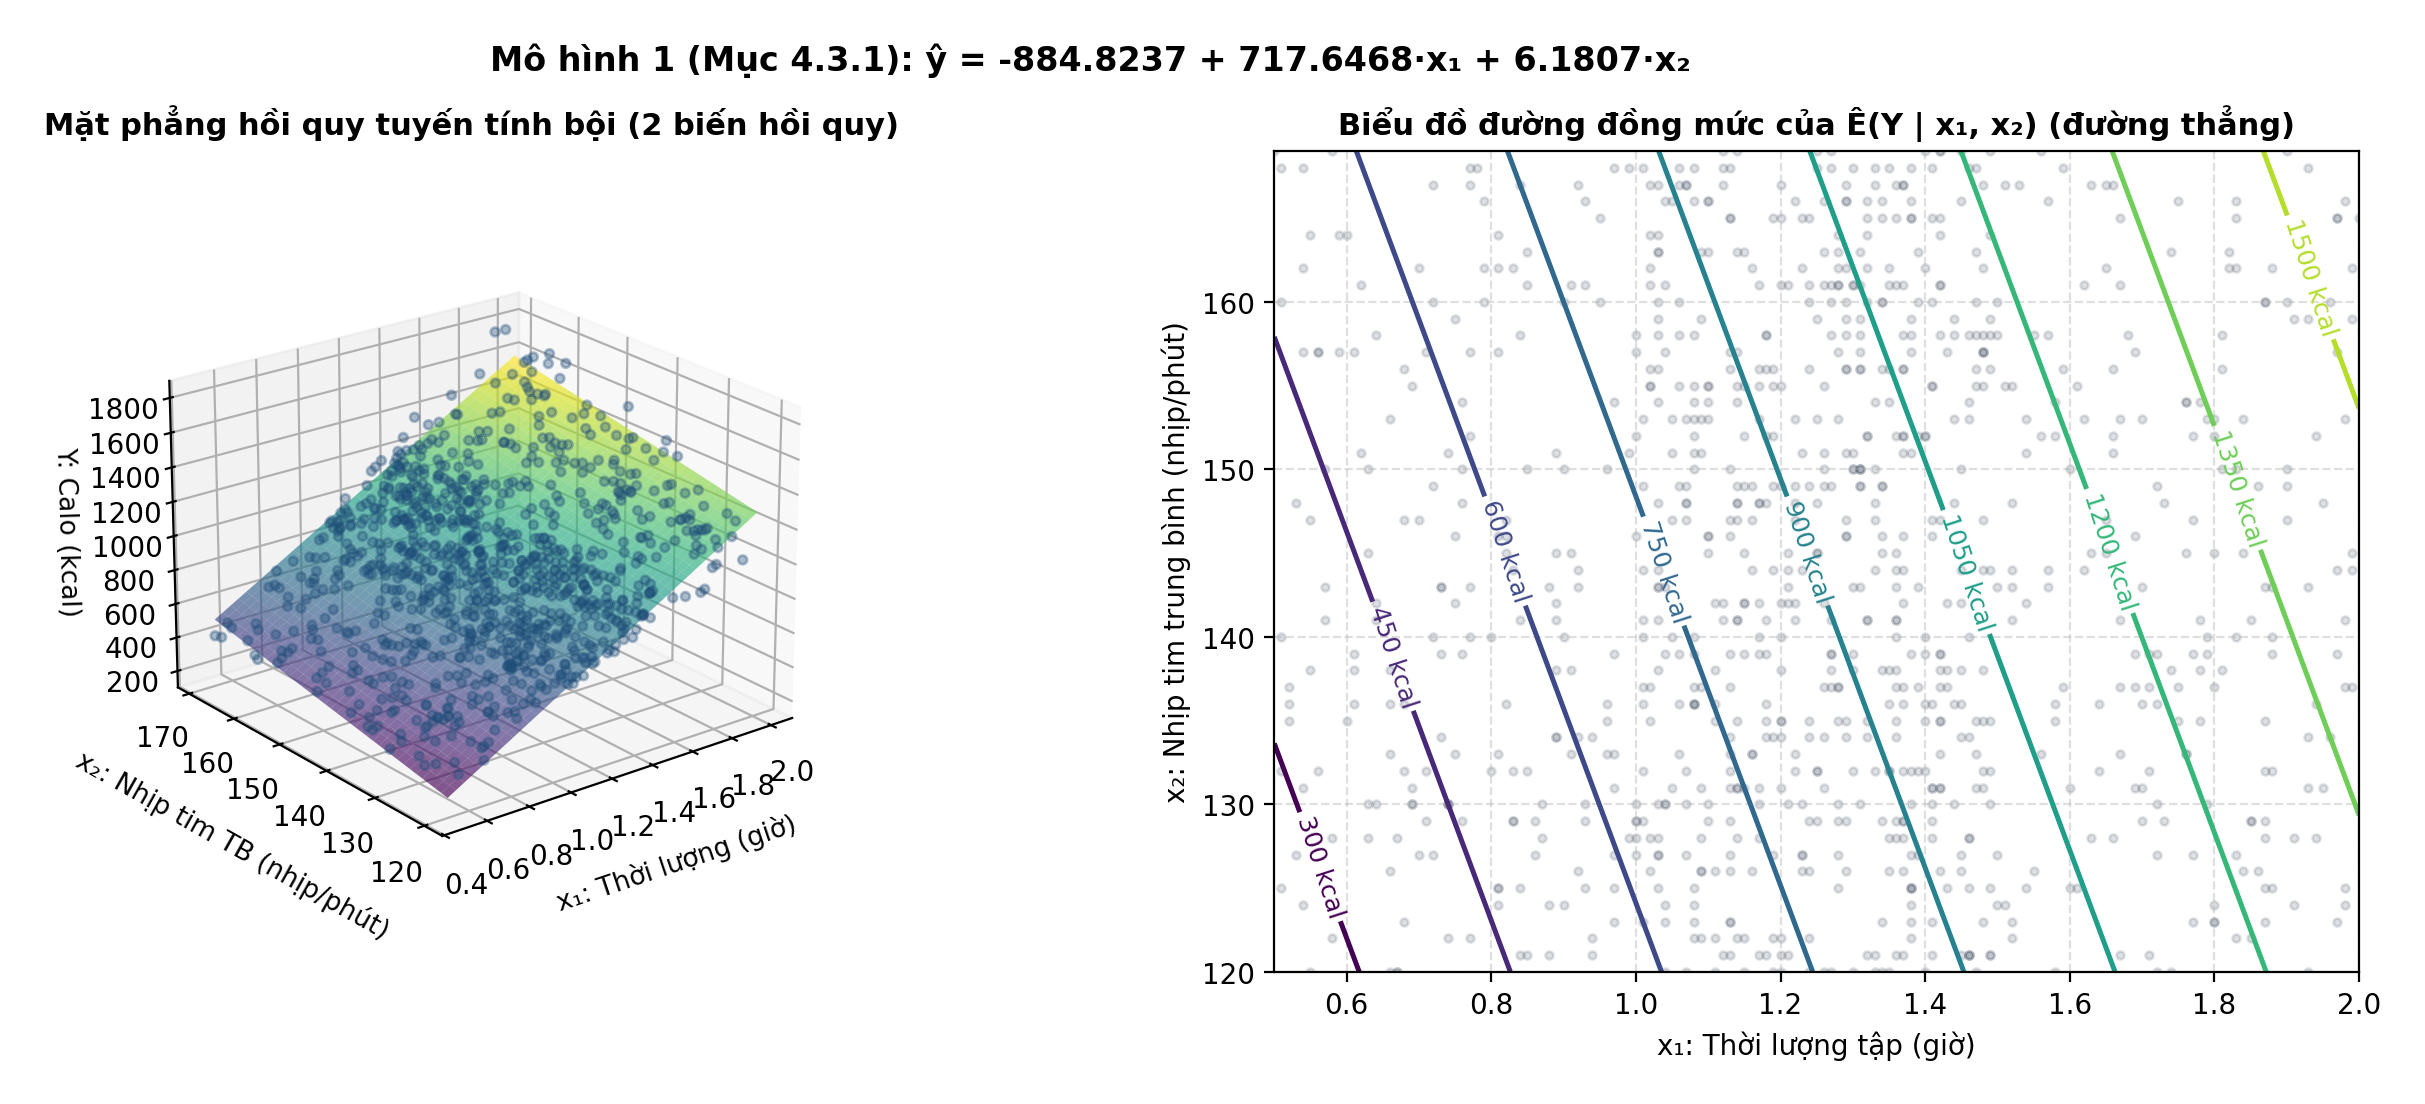
\includegraphics[width=0.96\textwidth]{../outputs/figures/07_mlr_plane_contour.png}
\caption{Mặt phẳng hồi quy 3D và biểu đồ đường đồng mức hai chiều của Mô hình 1 ($Y$ theo $x_1, x_2$)}
\label{fig:mlr_plane}
\end{figure}

\begin{figure}[htbp]
\centering
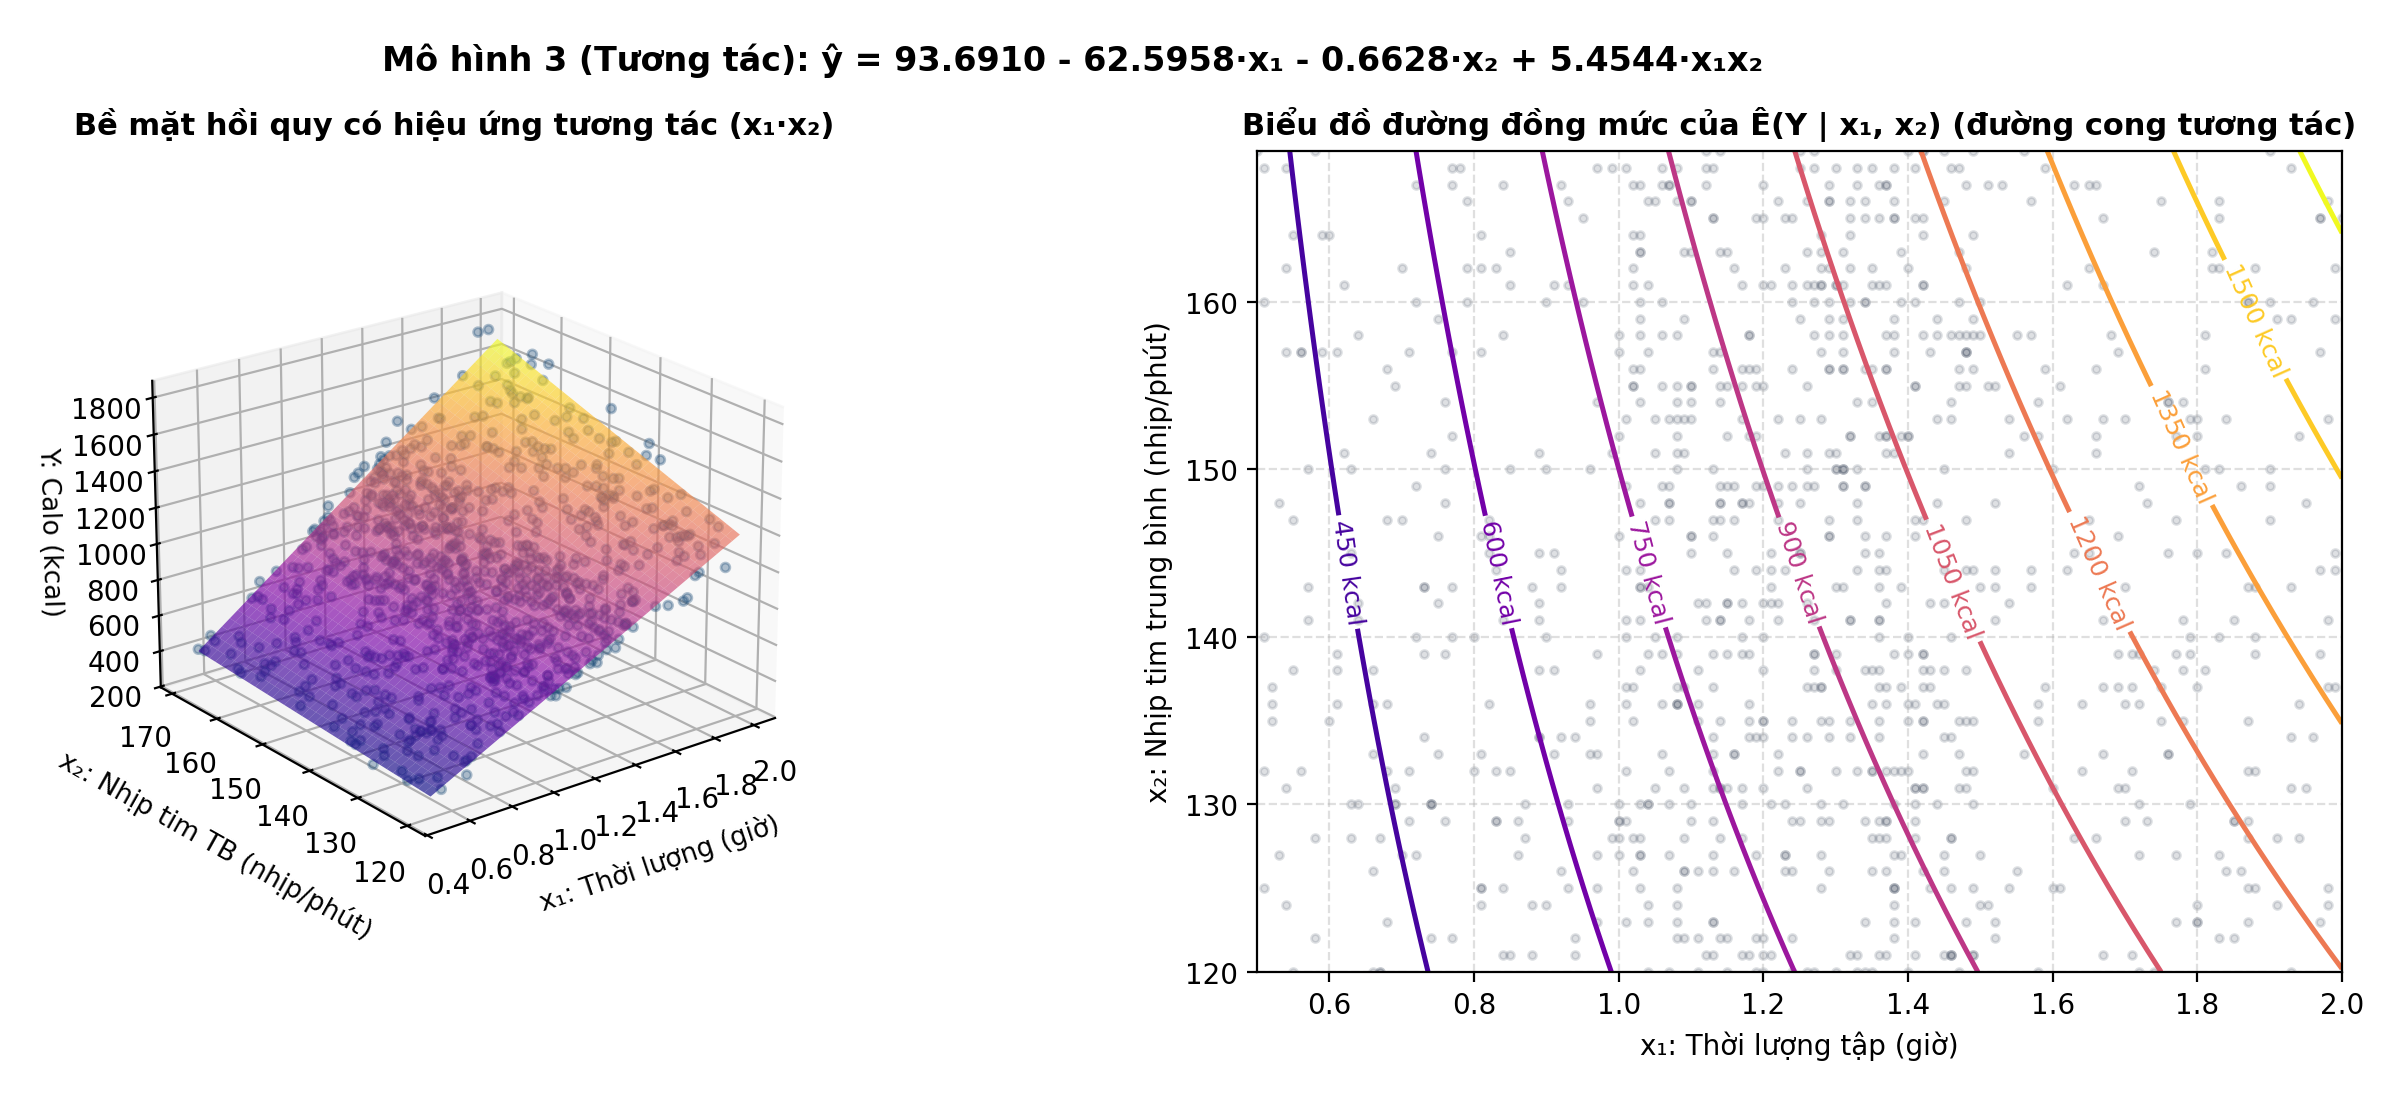
\includegraphics[width=0.96\textwidth]{../outputs/figures/07_mlr_interaction_surface.png}
\caption{Bề mặt hồi quy 3D và biểu đồ đường đồng mức của Mô hình 3 có hiệu ứng tương tác $x_1 x_2$}
\label{fig:mlr_interact}
\end{figure}

% ==================== CHƯƠNG 5 ====================
\chapter{Kết luận và hướng phát triển}
\section{Kết luận}
Báo cáo đã hoàn thành toàn diện các mục tiêu nghiên cứu của học phần Suy luận Thống kê:
\begin{enumerate}
    \item Khảo sát mẫu ngẫu nhiên $973$ thành viên phòng gym, kiểm tra tính toàn vẹn và lập bảng thống kê mô tả.
    \item Ước lượng điểm và xây dựng khoảng tin cậy 95\% (1 phía, 2 phía) cho kỳ vọng, phương sai, tỷ lệ và so sánh 2 tổng thể.
    \item Thực hiện quy trình kiểm định tham số và phi tham số bằng 3 cách tiếp cận nhất quán; chứng minh tác động của loại hình bài tập qua ANOVA ($P = 0.00016$).
    \item Xây dựng mô hình hồi quy tuyến tính đơn giải thích $82.47\%$ biến thiên lượng calo; chứng minh chặt chẽ $t_0^2 = f_0$, phân tích phần dư chuẩn hóa và biến đổi Fisher $Z$.
    \item Bổ sung mô hình hồi quy tuyến tính bội (Mục 4.3.1) và ước lượng các hệ số hồi quy riêng bằng phương pháp ước lượng bình phương nhỏ nhất thông qua hệ $p = k + 1$ phương trình chuẩn (Mục 4.3.2), minh họa trực quan mặt phẳng hồi quy, bề mặt tương tác và biểu đồ đường đồng mức.
\end{enumerate}

\section{Hướng phát triển: hồi quy tuyến tính bội}
Để kiểm soát đồng thời các biến giấu mặt, mô hình sẽ được mở rộng sang Hồi quy tuyến tính bội:
\[ \text{Calories\_Burned} = \beta_0 + \beta_1 \cdot \text{Session\_Duration} + \beta_2 \cdot \text{Avg\_BPM} + \beta_3 \cdot \text{Weight} + \sum_{j} \gamma_j \cdot I_{\text{Workout\_Type}_j} + \varepsilon \]
Mô hình mở rộng hứa hẹn nâng hệ số $R^2$ tiệm cận $95\%$ và cho phép phân tích độ co giãn calo theo nhịp tim và cân nặng.

% ==================== TÀI LIỆU THAM KHẢO ====================
\begin{thebibliography}{99}
\bibitem{walpole} Walpole, R. E., Myers, R. H., Myers, S. L., \& Ye, K. (2012). \textit{Probability \& Statistics for Engineers \& Scientists} (9th ed.). Boston: Pearson.
\bibitem{montgomery} Montgomery, D. C., \& Runger, G. C. (2018). \textit{Applied Statistics and Probability for Engineers} (7th ed.). Hoboken, NJ: John Wiley \& Sons.
\bibitem{sami} Viện Toán ứng dụng và Tin học, Đại học Bách khoa Hà Nội. (2024). \textit{Bài giảng Suy luận Thống kê (MI3031)}.
\bibitem{kaggle} Khorasani, V. (2024). \textit{Gym Members Exercise Dataset}. Kaggle Datasets.
\end{thebibliography}

\end{document}
